\documentclass[12pt]{article}
\author{Michael Vu}
\title{Numerical Analysis HW 7}
\usepackage{pdfsync} %This package allows for some communication between your pdf viewer and your latex editor, so that you can double click on a line in the pdf, for instance, and it will jump to the corresponding line in your latex code.

\usepackage{amssymb, amsmath, graphicx,amsthm} %these are standard packages that I pretty much always use.

\usepackage{bm,stmaryrd,verbatim,color,amsbsy}
%\usepackage{showkeys}  %If you have trouble remembering what you labeled your equations, you can uncomment this package, and temporarily see the labels displayed.
\usepackage{epstopdf} %Since I use Maple sometimes to make figures, and I get it to output eps files, I use this package so that eps files can be inputted into my documents. 
%Mathematica has the ability to output figures as pdfs, which are handled automatically with the graphicx package enabled.

\usepackage[normalem]{ulem} %this is a package that lets you underline, but mostly I like the \sout command for striking out.

\usepackage{color} %this package lets us change the color of your font by writing something like {\color[rgb]{1,0,0} This would be red}.




\def\red #1{{\color[rgb]{1, 0,0}#1}} %To make things easy on myself, I define a simpler function like this, so I can write \red{This would be red} instead of the above babble.

\newtheorem{theorem}{Theorem}[section]
\newtheorem{lemma}[theorem]{Lemma}
\newtheorem{proposition}[theorem]{Proposition}
\newtheorem{corollary}[theorem]{Corollary} %These define theorem like environments.

\newenvironment{definition}[1][Definition]{\begin{trivlist}
\item[\hskip \labelsep {\bfseries #1}]}{\end{trivlist}}
\newenvironment{example}[1][Example]{\begin{trivlist}
\item[\hskip \labelsep {\bfseries #1}]}{\end{trivlist}}
\newenvironment{remark}[1][Remark]{\begin{trivlist}
\item[\hskip \labelsep {\bfseries #1}]}{\end{trivlist}} %These define various other types of math environments: definition, example, and remarks.

\newcommand{\ph}{\varphi}






\bibliographystyle{plain}


%Some common or not so common symbols that I wanted shortcuts for.
\newcommand{\eps}{\varepsilon}
\newcommand{\ddt}{\frac{\mbox{d}}{\mbox{d}t}}
\newcommand{\dA}{\,\mbox{d}A}
\newcommand{\dv}{\,\mbox{d}v}
\def\dx{\, \mbox{d} x}
\newcommand{\ds}{\,\mbox{d}s}
\newcommand{\dz}{\,\mbox{d}z}
\def\dzeta{\,\mbox{d}\zeta}
\newcommand{\dl}{\,\mbox{d}l}
\renewcommand{\div}{\mbox{ div}}
\newcommand{\grad}{\mbox{ grad }}




%bold letters usually used to denote vectors matrices.
\def\bfa{\mathbf{a}}
\def\bfA{\mathbf{A}}
\def\bfb{\mathbf{b}}
\def\bfB{\mathbf{B}}
\def\bfc{\mathbf{c}}
\def\bfC{\mathbf{C}}
\def\bfd{\mathbf{d}}
\def\bfD{\mathbf{D}}
\def\bfe{\mathbf{e}}
\def\bfE{\mathbf{E}}
\def\bff{\mathbf{f}}
\def\bfF{\mathbf{F}}
\def\bfg{\mathbf{g}}
\def\bfG{\mathbf{G}}
\def\bfh{\mathbf{h}}
\def\bfH{\mathbf{H}}
\def\bfi{\mathbf{i}}
\def\bfI{\mathbf{I}}
\def\bfj{\mathbf{j}}
\def\bfJ{\mathbf{J}}
\def\bfk{\mathbf{k}}
\def\bfK{\mathbf{K}}
\def\bfl{\mathbf{l}}
\def\bfL{\mathbf{L}}
\def\bfm{\mathbf{m}}
\def\bfM{\mathbf{M}}
\def\bfn{\mathbf{n}}
\def\bfN{\mathbf{N}}
\def\bfo{\mathbf{o}}
\def\bfO{\mathbf{O}}
\def\bfp{\mathbf{p}}
\def\bfP{\mathbf{P}}
\def\bfq{\mathbf{q}}
\def\bfQ{\mathbf{Q}}
\def\bfr{\mathbf{r}}
\def\bfR{\mathbf{R}}
\def\bfs{\mathbf{s}}
\def\bfS{\mathbf{S}}
\def\bft{\mathbf{t}}
\def\bfT{\mathbf{T}}
\def\bfu{\mathbf{u}}
\def\bfU{\mathbf{U}}
\def\bfv{\mathbf{v}}
\def\bfV{\mathbf{V}}
\def\bfw{\mathbf{w}}
\def\bfW{\mathbf{W}}
\def\bfx{\mathbf{x}}
\def\bfX{\mathbf{X}}
\def\bfy{\mathbf{y}}
\def\bfY{\mathbf{Y}}
\def\bfz{\mathbf{z}}
\def\bfZ{\mathbf{Z}}



%``Blackboard bold" letters \bbC is used for the complex plane, \bbN
\def\bba{\mathbb{a}}
\def\bbA{\mathbb{A}}
\def\bbb{\mathbb{b}}
\def\bbB{\mathbb{B}}
\def\bbc{\mathbb{c}}
\def\bbC{\mathbb{C}}
\def\bbd{\mathbb{d}}
\def\bbD{\mathbb{D}}
\def\bbe{\mathbb{e}}
\def\bbE{\mathbb{E}}
\def\bbf{\mathbb{f}}
\def\bbF{\mathbb{F}}
\def\bbg{\mathbb{g}}
\def\bbG{\mathbb{G}}
\def\bbh{\mathbb{h}}
\def\bbH{\mathbb{H}}
\def\bbi{\mathbb{i}}
\def\bbI{\mathbb{I}}
\def\bbj{\mathbb{j}}
\def\bbJ{\mathbb{J}}
\def\bbk{\mathbb{k}}
\def\bbK{\mathbb{K}}
\def\bbl{\mathbb{l}}
\def\bbL{\mathbb{L}}
\def\bbm{\mathbb{m}}
\def\bbM{\mathbb{M}}
\def\bbn{\mathbb{n}}
\def\bbN{\mathbb{N}}
\def\bbo{\mathbb{o}}
\def\bbO{\mathbb{O}}
\def\bbp{\mathbb{p}}
\def\bbP{\mathbb{P}}
\def\bbq{\mathbb{q}}
\def\bbQ{\mathbb{Q}}
\def\bbr{\mathbb{r}}
\def\bbR{\mathbb{R}}
\def\bbs{\mathbb{s}}
\def\bbS{\mathbb{S}}
\def\bbt{\mathbb{t}}
\def\bbT{\mathbb{T}}
\def\bbu{\mathbb{u}}
\def\bbU{\mathbb{U}}
\def\bbv{\mathbb{v}}
\def\bbV{\mathbb{V}}
\def\bbw{\mathbb{w}}
\def\bbW{\mathbb{W}}
\def\bbx{\mathbb{x}}
\def\bbX{\mathbb{X}}
\def\bby{\mathbb{y}}
\def\bbY{\mathbb{Y}}
\def\bbz{\mathbb{z}}
\def\bbZ{\mathbb{Z}}

\def\ca{\mathcal{a}}
\def\cA{\mathcal{A}}
\def\cb{\mathcal{b}}
\def\cB{\mathcal{B}}
\def\cc{\mathcal{c}}
\def\cC{\mathcal{C}}
\def\cd{\mathcal{d}}
\def\cD{\mathcal{D}}
\def\ce{\mathcal{e}}
\def\cE{\mathcal{E}}
\def\cf{\mathcal{f}}
\def\cF{\mathcal{F}}
\def\cg{\mathcal{g}}
\def\cG{\mathcal{G}}
\def\ch{\mathcal{h}}
\def\cH{\mathcal{H}}
\def\ci{\mathcal{i}}
\def\cI{\mathcal{I}}
\def\cj{\mathcal{j}}
\def\cJ{\mathcal{J}}
\def\ck{\mathcal{k}}
\def\cK{\mathcal{K}}
\def\cl{\mathcal{l}}
\def\cL{\mathcal{L}}
\def\cm{\mathcal{m}}
\def\cM{\mathcal{M}}
\def\cn{\mathcal{n}}
\def\cN{\mathcal{N}}
\def\co{\mathcal{o}}
\def\cO{\mathcal{O}}
\def\cp{\mathcal{p}}
\def\cP{\mathcal{P}}
\def\cq{\mathcal{q}}
\def\cQ{\mathcal{Q}}
\def\calr{\mathcal{r}}
\def\cR{\mathcal{R}}
\def\cs{\mathcal{s}}
\def\cS{\mathcal{S}}
\def\ct{\mathcal{t}}
\def\cT{\mathcal{T}}
\def\cu{\mathcal{u}}
\def\cU{\mathcal{U}}
\def\cv{\mathcal{v}}
\def\cV{\mathcal{V}}
\def\cw{\mathcal{w}}
\def\cW{\mathcal{W}}
\def\cx{\mathcal{x}}
\def\cX{\mathcal{X}}
\def\cy{\mathcal{y}}
\def\cY{\mathcal{Y}}
\def\cz{\mathcal{z}}
\def\cZ{\mathcal{Z}}

%Some operators that I wanted displayed in a similar font as you would want sin and cos functions (by the way, those can be called up by using \sin,\cos,\log,\ln, \tan,\exp,\sec,\csc,\sinh,\cosh,\tanh, there are probably more.
\DeclareMathOperator*{\sgn}{sgn}
\DeclareMathOperator*{\spn}{span}
\DeclareMathOperator*{\coker}{coker}
\DeclareMathOperator*{\Id}{Id}
\DeclareMathOperator*{\D}{D}
\def\RR{\mathbb{R}}

%more symbols that I wanted extra short commands for
\newcommand{\be}{\mathbf{e}}
\renewcommand{\L}{\Lambda}
\newcommand{\vs}{\varsigma}
\newcommand{\al}{\alpha}
\newcommand{\s}{\sigma}
\renewcommand{\k}{\kappa}
\renewcommand{\t}{\theta}
\newcommand{\w}{\omega}


%some bold greek letters.
\def\bfeta{\boldsymbol{\eta}}
\def\bfxi{\boldsymbol{\xi}}
\def\bfrho{\boldsymbol{\rho}}
\def\bfth{\boldsymbol{\t}}
\def\bflam{\boldsymbol{\lambda}}
\def\bfTh{\boldsymbol{\Theta}}
\def\bfnu{\boldsymbol{\nu}}

\newcommand{\drho}{\,{\rm d} \rho}
\newcommand{\dth}{\,{\rm d} \t}
\newcommand{\tilu}{\tilde{u}}
\newcommand{\vt}{\vartheta}


\begin{document}

\maketitle 

\textbf{Problem 1.} We are asked to solve problem 7 of section 5.6. Below is the ODE driver for solving the problem:

\begin{verbatim}
implicit none
double precision :: t,tout,relerr,abserr,a,b,dt
double precision, allocatable, dimension(:) :: y(:), work(:)
integer, allocatable, dimension(:) :: iwork(:)
integer :: nsteps,i,iflag,neqn
external f

neqn = 1

allocate( y(neqn), work(100+21*neqn), iwork(5) )

y = (/ 0.0d0 /)
a = 0.0d0
b = 2.0d0
nsteps = 100
t = a
dt = (b-a)/dble(nsteps)
relerr = 1.0d-10
abserr = 1.0d-10
iflag = 1

do i = 1,nsteps
	tout = t + dt
	call ode(f,neqn,y,t,tout,relerr,abserr,iflag,work,iwork)
	
	if(iflag /= 2) then
		print*, 'Warning: i, iflag = ', i, iflag
	end if
	
	print*, tout, y(1)
end do

deallocate(y,work,iwork)
stop
end

subroutine f(t,y,yp)
implicit none
double precision :: t,y(1),yp(1)

yp(1) = (110.d0 * cos(t) - y(1)) / (1.1d0 * (2.1d0 + 1.8d0 * y(1)))


return
end
\end{verbatim}

These are the first and last few interations leading up to $t=2$:

\begin{verbatim}
t=                        i(t)=
2.0000000000000000E-002   0.72417563949512709
4.0000000000000001E-002   1.2367583733012615
5.9999999999999998E-002   1.6558366962986306
.
.
.
1.9600000000000013        8.3226127553865492
1.9800000000000013        8.2681151148920353
2.0000000000000013        8.2111871600797919 
\end{verbatim}

So we find that $i(2)$ is approximately 8.211871600797919. Below is the graph as we travel forward in time from 0 to 2:

\begin{figure}[htbp]
	\centering
		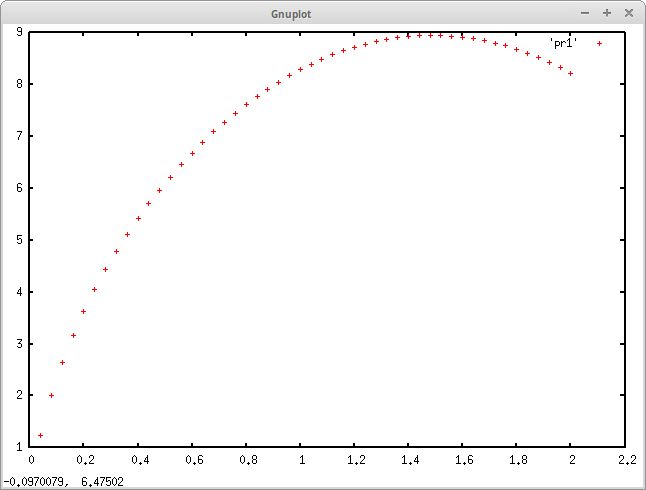
\includegraphics[width=1.00\textwidth]{hw7pr1graph.png}
	\label{fig:hw7pr1graph}
\end{figure}

\textbf{Problem 2.} We are asked to solve problem 5 of section 5.5. Below is the ODE driver to solve the problem:

\begin{verbatim}
implicit none
double precision :: t,tout,relerr,abserr,a,b,dt
double precision, allocatable, dimension(:) :: y(:), work(:)
integer, allocatable, dimension(:) :: iwork(:)
integer :: nsteps,i,iflag,neqn
external f

neqn = 1

allocate( y(neqn), work(100+21*neqn), iwork(5) )

y = (/ 50976.0d0 /)
a = 0.0d0
b = 5.0d0
nsteps = 100
t = a
dt = (b-a)/dble(nsteps)
relerr = 1.0d-10
abserr = 1.0d-10
iflag = 1

do i = 1,nsteps
	tout = t + dt
	call ode(f,neqn,y,t,tout,relerr,abserr,iflag,work,iwork)
	
	print*, tout, y(1)
	
	if(iflag /= 2) then
		print*, 'Warning: i, iflag = ', i, iflag
	stop
	end if
end do

deallocate(y,work,iwork)
stop
end

subroutine f(t,y,yp)
implicit none
double precision :: t,y(1),yp(1)

yp(1) = 2.9d-2 * y(1) - 1.4d-7 * (y(1)**2)

return
end
\end{verbatim}

These are the first and last few interations leading up to $t=5$:

\begin{verbatim}
t=                        P(t)=
5.0000000000000003E-002   51031.745846037498
0.10000000000000001       51087.532711320688
0.15000000000000002       51143.360582430090
.
.
.
4.8999999999999906        56631.626639862254
4.9499999999999904        56691.312111451043
4.9999999999999902        56751.036768758218
\end{verbatim}

So we find that $P(5)$ is approximately 56751.036768758218.

\bigskip

\textbf{Problem 3.} In this problem we are asked to solve an initial value problem given by Dr. Glunt, this is the ODE driver use to solve this problem:

\begin{verbatim}
implicit none
double precision :: t,tout,relerr,abserr,a,b,dt
double precision, allocatable, dimension(:) :: y(:), work(:)
integer, allocatable, dimension(:) :: iwork(:)
integer :: nsteps,i,iflag,neqn
external f

neqn = 2

allocate( y(neqn), work(100+21*neqn), iwork(5) )

y = (/ 1.0d0,0.0d0 /)
a = 0.0d0
b = 10.0d0
nsteps = 100
t = a
dt = (b-a)/dble(nsteps)
relerr = 1.0d-10
abserr = 1.0d-10
iflag = 1

do i = 1,nsteps
	tout = t + dt
	call ode(f,neqn,y,t,tout,relerr,abserr,iflag,work,iwork)
	
	print*, t, y(1)
	
	if(iflag /= 2) then
		print*, 'Warning: i, iflag = ', i, iflag
	stop
	end if
end do

deallocate(y,work,iwork)
stop
end

subroutine f(t,y,yp)
implicit none
double precision :: t,y(2),yp(2)

yp(1) = y(2)
yp(2) = -1.0d0 / (y(1)**2)

return
end
\end{verbatim}

This is the output from the code:

\begin{verbatim}
t=                        z(t)=
0.10000000000000001       0.99499163596971130
0.20000000000000001       0.97986467324765869
0.30000000000000004       0.95430172599537555
0.40000000000000002       0.91773111353375358
0.50000000000000000       0.86924869765427382
0.59999999999999998       0.80747099501982766
0.69999999999999996       0.73024958947622853
0.79999999999999993       0.63405965896115235
0.89999999999999991       0.51244965313027724
0.99999999999999989       0.35068159575822078
1.0999999999999999        7.8972465069453615E-002
1.1107207348315986        2.7160802790846351E-008
Warning: i, iflag =  12, 4
\end{verbatim}

It appears to have had an error when running the program. Since this problem sets up a scenario where two stars are on a collision path, the point in time which we receive this error indicates a collision as occured. 

\bigskip

\textbf{Problem 4.} This problem is similar to problem 3. The only change that was made was to halt the program when $z\leq 0.01$. Problem 3 sets up a collision between the stars as point particles rather than an object that actually takes some space. Setting up the problem in this new manner should simulate a better scenario of two stars colliding. This is the ODE driver used to solve this problem:

\begin{verbatim}
implicit none
double precision :: t,tout,relerr,abserr,a,b,dt
double precision, allocatable, dimension(:) :: y(:), work(:)
integer, allocatable, dimension(:) :: iwork(:)
integer :: nsteps,i,iflag,neqn
external f

neqn = 2

allocate( y(neqn), work(100+21*neqn), iwork(5) )

y = (/ 1.0d0,0.0d0 /)
a = 0.0d0
b = 10.0d0
nsteps = 100
t = a
dt = (b-a)/dble(nsteps)
relerr = 1.0d-10
abserr = 1.0d-10
iflag = 1

do i = 1,nsteps
	tout = t + dt
	call ode(f,neqn,y,t,tout,relerr,abserr,iflag,work,iwork)
	
	print*, t, y(1)
	
	if(y(1) <= 0.01d0) then
		print*, 'Collision has occured'
	stop
	end if	
	
	if(iflag /= 2) then
		print*, 'Warning: i, iflag = ', i, iflag
	stop
	end if
end do

deallocate(y,work,iwork)
stop
end

subroutine f(t,y,yp)
implicit none
double precision :: t,y(2),yp(2)

yp(1) = y(2)
yp(2) = -1.0d0 / (y(1)**2)

return
end
\end{verbatim}

This is the output from the code:

\begin{verbatim}
t=                        z(t)=
0.10000000000000001       0.99499163596971130
0.20000000000000001       0.97986467324765869
0.30000000000000004       0.95430172599537555
0.40000000000000002       0.91773111353375358
0.50000000000000000       0.86924869765427382
0.59999999999999998       0.80747099501982766
0.69999999999999996       0.73024958947622853
0.79999999999999993       0.63405965896115235
0.89999999999999991       0.51244965313027724
0.99999999999999989       0.35068159575822078
1.0999999999999999        7.8972465069453615E-002
1.1107207348315986        2.7160802790846351E-008
Collision has occured
\end{verbatim}

This should have resulted in different stopping times, however, it did not. This is either an error on my part, or something else. In either case, the output stopped when $z(t=1.1107207348315986)= 2.7160802790846351\times10^{-8}$

\end{document}